\section{PAC Learning}
\label{sec:pac-learning}
\begin{enumerate}

\item ~[15 points] Due to the recent budget cuts the government no
  longer has any money to pay for humans to monitor the state of
  nuclear reactors. They have charged you with assessing a Robot's
  ability to perform this vital task. Every reactor has a different
  number of binary gauges which indicate whether or not some aspect of
  the reaction is {\tt normal} or {\tt strange}. The reactor itself
  can be in one of {\bf five} states -- {\em Normal}, {\em Meltdown},
  {\em Pre-meltdown}, {\em Abnormally cool} or {\em Off}. Each
  combination of the binary guage settings indicate one of these five
  reactor states. We want to know if we can train a robot to identify
  which gauges and gauge combinations are responsible for each reactor
  state.

  \begin{enumerate}
  \item [a)][5 points] Suppose that we have $N$ gauges with which to
    identify reactor states. How large is the hypothesis space for
    this task? (You may have to make assumptions about the underlying
    function space. State your assumptions clearly.)

\begin{itemize}
  \item We can {\em assume} that since this is a nuclear reactor that all of the gauges are important, and thus there are $3^{N}$ different conjunctions for determining the state of the nuclear reactor.%Where $K$ is the number of gauges that need to be looked at, we can say there is a hypothesis space of ${N \choose K}$. For this to be true, we have to assume that there are no repetitions. Or, we can {\em assume} that since this is a nuclear reactor, all of the gauges are important so there is $3^{N}$ different conjunctions for determining the states.
\end{itemize}

  \item[b)] [10 points] The ex-government employee, whose job the
    robot is taking, trains the robot at a nuclear reactor where there
    are 20 gauges by showing the robot a set of gauge positions for
    the five different reactor states. If the robot wants to learn to
    recognize the reactor's condition with .1 percent error with
    greater than 99\% probability how many examples does the robot
    need to see?
\begin{itemize}
\item The following equation represents the relation for PAC learning
\begin{align*}
\delta &\geq He^{-\epsilon R}\\
\intertext{Where $R$ is the number of required training examples, $\epsilon$ is the error, and $\delta$ is the probability. We can solve for $R$ to get the maximum number of training examples.}
\frac{1}{\epsilon}\log\left( {\frac{\delta}{H}}\right) &\geq -R\\
\frac{1}{\epsilon}\log\left( {\frac{H}{\delta}}\right) &\geq R\\
\frac{1}{\epsilon}\left[n\log(3) - \log(\delta) \right] &\geq R\\
\intertext{where $\delta$ is defined as $(1-\text{probability})$ and $\epsilon$ is defined as $(1-\text{accuracy})$. We can plug these in from the stated problem and we get}
\frac{1}{0.10}\left(20\log(3) - \log(0.01) \right) &\geq R\\
R &\leq 266
\end{align*}
\end{itemize}

  \end{enumerate}


\item ~[5 points] Is it possible for a learned hypothesis $h$ to
   achieve 100\% accuracy with respect to a training set and still
   have non-zero true error? If so, provide a description of how this
   is possible. If not, prove that it is impossible.

\begin{itemize}
\item Yes, an instance of this would be when the data is overfit to the training data, which would result in 100\% accuracy on the training set and a large (non-zero) error on the test set, which would result in a non-zero true error.
\end{itemize}


\item ~[25 points] {\bf Learning decision lists:}
  In this problem, we are going to learn the class of $k$-decision
lists. A decision list is an ordered sequence of if-then-else
statements. The sequence of if-then-else conditions are tested in
order, and the answer associated to the first satisfied condition is
output. See Figure~\ref{fig:decision_list} for an example of a
$2$-decision list.

\begin{figure}[!h]
\begin{center}
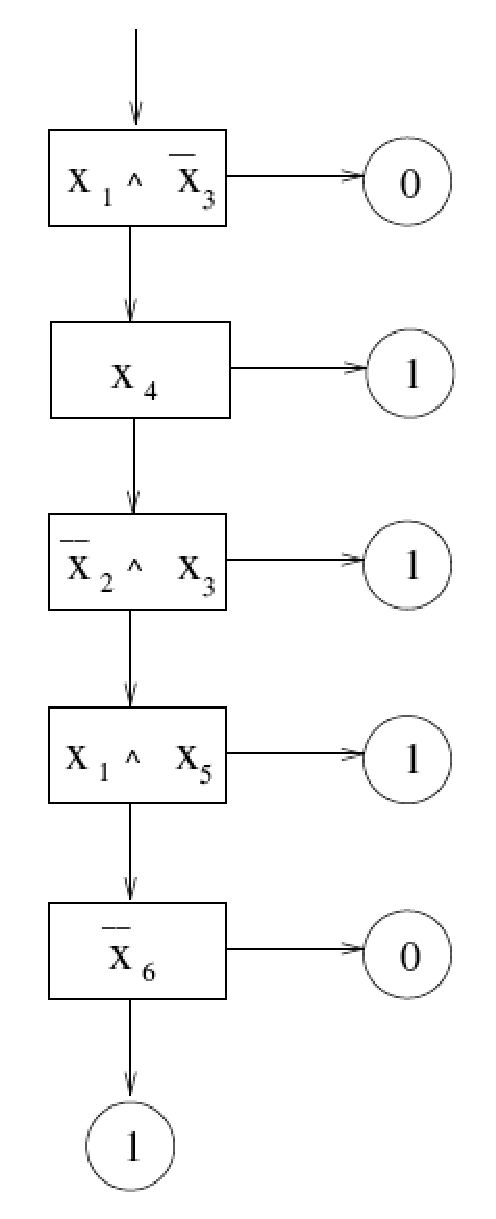
\includegraphics[width=1.35in]{fig-1.pdf}
\caption{A $2$-decision list.}
\label{fig:decision_list}
\end{center}
\end{figure}

A {\em $k$-decision list} over the variables $x_{1}, \ldots, x_{n}$ is
an ordered sequence $L=(c_{1}, b_{1}), \ldots, (c_{\ell},b_{\ell})$ and a
bit $b$, in which each $c_{i}$ is a conjunction of at most $k$
literals over $x_{1},\ldots, x_{n}$. The bit $b$ is called the {\em
  default} value, and $b_{i}$ is referred to as the bit {\em
  associated} with condition $c_{i}$. For any input $x \in \{0,
1\}^{n}$, $L(x)$ is defined to be the bit $b_{j}$, where $j$ is the
smallest index satisfying $c_{j}(x)=1$; if no such index exists, then
$L(x)=b$.

We denote by $k\mbox{\em -DL}$ the class of concepts that can be
represented by a $k$-decision list.


\begin{enumerate}
\item \relax[8 points] Show that if a concept $c$ can be represented
  as a $k$-decision list so can its complement, $\neg c$. You can show
  this by providing a $k$-decision list that represents $\neg c$,
  given $c = \{(c_{1},b_{1}), \ldots, (c_{\ell},b_{\ell}),b\}$.

\begin{itemize}
\item To prove that the complement of $c$ is a $k$-decision list, we can simply take $c$ and negate all of the bits to produce another $k$-decision list. It would look such as the following: $\neg c = \{(c_{1},\neg b_{1}), \ldots, (c_{\ell},\neg b_{\ell}),\neg b\}$, which is a $k$-decision list.
\end{itemize}
\item \relax[9 points] Use  Occam's Razor to show: \\
  For any constant $k \geq 1$, the class of $k$-decision lists is
  PAC-learnable.

\begin{itemize}
\item Occam's Razor states that the least complicated case is most likely true, but in this course we take it as being true. Therefore, we can show this to be PAC-learnable by finding a lower bound on the set such that it is the minimum $k$-decision list. This can be done by showing that the dimensions of data needed is {\em finite}.

It can be trivially seen that the size of the concept class is $\left| c_{k} \right| = \mathcal{O}\left( n^{k}\right)$. Each of the bits belong in $b_{i}\in \{ 0,1 \}$, and since there are $\ell$ of them it results in $2^{\ell}$ different combinations. There are also $\ell!$ orderings of those bits. Finally, the size of the concept class that can describe the data is $2^{\left| c_{k} \right|}$. Therefore, the overall bound is represented by the product of these three which is $\mathcal{O}\left( 2^{\left| c_{k} \right|}\cdot \ell!\cdot 2^{\ell} \right)$. However, the {\em maximum value} of $\ell$ is represented by $\left| c_{k} \right|$, so we can simplify our notation as $\mathcal{O}\left( 2^{2\left| c_{k}\right|}\left| c_{k} \right|!\right)$.

Finally, the size of the number of examples needed in our set is logarithmically proportional to the size of the concept class, so by taking the log we get $\mathcal{O}\left( 2n^{k}\log(2) + kn^{k}\log(n)\right)$ which is a {\em finite number} for any $k\geq 1$ and thus is PAC-learnable.
\end{itemize}
\item \relax[8 points] Show that $1$-decision lists are a linearly
  separable functions. (Hint: Find a weight vector that will make the
  same predictions a given $1$-decision list.)

\begin{itemize}
\item To do this, we need to construct our $\mathbf{x}$ vector and then our $\mathbf{w}$ vector where $\mathbf{w}$ is the weight vector defined as $\mathbf{w} = (\theta , w_{1}, w_{2}, \ldots , w_{\ell})^{T}$ with $\theta$ being the bias. We can define our $\mathbf{x}$ vector as $\mathbf{x} = (1, x_{1}, x_{2}, \ldots, x_{\ell})^{T}$ with the leading term being needed to support the bias. $x_{i}$ can be defined by the value of $b_{i}$, where $x_{i} = -1$ for $b_{i} = 0$, and $x_{i} = 1$ for $b_{i} = 1$. From here, we can create a threshold function to ``learn'' the $k$-decision list, which is defined as $\mathbf{w}^{T}\cdot \mathbf{x} \geq 0$.

In building $\mathbf{w}$, we can define each element of $w_{i} = b_{i}\cdot 2^{\ell+1-i}$ as to separate the individual data points. This would make the first few elements $\mathcal{O}\left(\pm 2^{\ell}\right)$ and the last elements $\mathcal{O}(\pm 2)$, where the $\pm$ comes about due to the individual bit $b_{i}$. Following this, we can look at the original 1-DL and if the overall/default bit is false, then we can set $\theta = -1$, else $\theta = 1$. This would overall be equivalent to the 1-DL and would make it liearly separable and learnable.
\end{itemize}
\end{enumerate}



%%% Local Variables: 
%%% mode: latex
%%% TeX-master: "hw3"
%%% End: 


\item ~[20 points, {\bf CS 6350 students only}] Let $X$ be an instance
  space and let $D_1,D_2,...,D_m$ be a sequence of distributions over
  $X$. Let $\mathcal{H}$ be a finite class of binary classifiers over
  $X$ and let $f\in \mathcal{H}$. 

  Suppose we have a sample $S$ of $m$ examples, such that the
  instances are independent but are not identically distributed. The
  $i^{th}$ instance is sampled from $D_i$ and then $y_i$ is set to be
  $f(x_i)$. Let $\bar{D}_m$ denote the average, that is,
  $\bar{D}_m = \frac{1}{m}\sum_{i=1}^m D_i$. 

  Let $h \in \mathcal{H}$ be a classifier that gets zero error on the
  training set. That is, for every example $x_i \in X$, we have
  $h(x_i) = f(x_i)$. Show that, for any accuracy parameter
  $\epsilon \in (0, 1)$, the probability that the expected error of
  the learned classifier $h$ is greater than $\epsilon$ is no more
  than $|\mathcal{H}|e^{-\epsilon m}$. That is, show that

  \[\mathbb{P}\left[E_{x \sim \bar{D}_m}\left[h(x) \ne f(x)\right]> \epsilon\right] \leq  |\mathcal{H}|e^{-\epsilon m}\]

  (Hint: You have to use the fact that the arithmetic mean of a set of
  non-negative numbers greater than or equal to their geometric mean.)

\begin{itemize}
\item We can say that the expection value of the function is defined as
\begin{align*}
E_{x \sim \bar{D}_m}(\mathbb{I}_{\{h(x) = f(x)\}}) &= E_{x\sim \bar{D}_m}(\mathbb{Z}(x))\\
\intertext{Where the second relation is the same but $\mathbb{Z}(x)$ was introduced to shorten notation. We can say that this relation is equivalent to}
E_{x\sim \bar{D}_m}(\mathbb{Z}(x)) &= \underbrace{\sum_{x}\bar{D}(x)}_{\frac{1}{m}\sum_{i=1}^{m}D_{i}(x)}\mathbb{Z}(x) = \frac{1}{m}\sum_{x}\sum_{i=1}^{m}D_{i}(x)\mathbb{Z}(x)
\intertext{From here, we can switch the summations}
&= \frac{1}{m}\sum_{i=1}^{m}\underbrace{\sum_{x}D_{i}(x)\mathbb{Z}(x)}_{E_{x\sim D_{i}}} = \frac{1}{m}\sum E_{x\sim D_{i}}\mathbb{Z}(x)\quad (1)\\
\intertext{From the above problem, we can see that it's an independent distribution of probabilities, though it is not uniform. Therefore, we have the total probability as being}
P\left( \mathbb{Z}(x_{i})\ \forall i\right) &= \prod_{i=1}^{m}P\left( \mathbb{Z}(x_{i}) \right) \leq \left( \frac{1}{m}\sum_{i=1}^{m}P\left( \mathbb{Z}(x_{i})\right) \right)^{m} \quad (2)
\intertext{Where $(2)$ comes about because $\frac{1}{m}\sum_{i=1}^{m}x_{i} \geq \left( \prod_{i=1}^{m}x_{i} \right)^{\frac{1}{m}}$. By plugging $(1)$ into $(2)$, we get}
&= \left( \frac{1}{m}\sum_{i=1}^{m}E_{x\sim D_{i}}\left[ \mathbb{Z}(x)\right] \right)^{m} < (1-\epsilon)^{m}\\
\intertext{From here we can say that $(1-x) < e^{-x}$ as $(1-x)$ is a first order taylor series expansion of $e^{-x}$. Therefore, we reduce it to the following relation}
 &< e^{-m\epsilon}\\
\intertext{Where we can then apply the {\em Union Bound}, which states that the probability of at least one event happening is less than the sum of the probabilities of the individual events.}
&< \left| H \right|e^{-m\epsilon}
\end{align*}
\end{itemize}
\end{enumerate}

%%% Local Variables:
%%% mode: latex
%%% TeX-master: "hw3"
%%% End:
